\documentclass[xetex]{beamer}

\usepackage{fontspec}
%\usepackage{xeCJK}
%\setCJKmainfont{Noto Sans CJK SC}
%\newfontfamily\Libertine[Mapping=tex-text]{Linux Libertine O}
\usetheme{Madrid}
\usecolortheme{crane}
\usepackage{graphicx}

\usepackage{polyglossia}
\setdefaultlanguage{english}
\newfontfamily\englishfont[Ligatures=NoCommon]{Linux Libertine O}
\setotherlanguage{arabic}
\newfontfamily\arabicfontsf[Script=Arabic]{Noto Naskh Arabic}
\setotherlanguage{chinese}
\newfontfamily\chinesefontsf[Script=CJK]{Noto Sans CJK SC}
\setotherlanguage{yue}
\newfontfamily\yuefontsf[Script=CJK]{Noto Sans CJK TC}

\setotherlanguage{japanese}
\newfontfamily\japanesefontsf[Script=CJK]{Noto Sans CJK JP} % Japanese font
\setotherlanguage{korean}
\newfontfamily\koreanfontsf[Script=CJK]{Noto Sans CJK KR} 
\setotherlanguage{thai}
\newfontfamily\thaifontsf[Script=Thai]{Noto Sans Thai}

\newfontfamily{\silipa}{Noto Serif}
\newcommand{\IPA}[1]{{\silipa\selectfont #1}}

% \newfontfamily\fontarabic[Script=Arabic]{Noto Naskh Arabic } 
% \newfontfamily\textchinese[Script=CJK]{Noto Sans CJK SC}
% \newfontfamily\textjapanese[Script=CJK]{Noto Sans CJK JP} % Japanese font
% \newfontfamily\textkorean[Script=CJK]{Noto Sans CJK KR} 
% \newfontfamily\textthai[Script=Thai]{Noto Sans Thai} % Thai font
% \newcomand{\textarabic}[1]{\begin{RTL}\fontarabic\selectfont #1\end{RTL}}

\usepackage{mygb4e}
\newcommand{\yueb}[1]{\yuefontsf\selectfont #1}
\renewcommand{\eachwordone}{\yueb}
\renewcommand{\eachwordtwo}{\yueb}
\usepackage[e,f]{mtg2e}
\usepackage{xcolor}
\renewcommand{\mtcitestyle}[1]{\textcolor{teal}{\textit{#1}}}
\newcommand{\msa}{\mtciteform}
\newcommand{\zsm}{\mtciteform}
\newcommand{\ko}{\mtciteform}
\newcommand{\zh}{\mtciteform}
\newcommand{\jpn}{\mtciteform}
\newcommand{\ar}{\mtciteform}
\newcommand{\txx}[1]{\textcolor{blue}{\textbf{#1}}}

\title{Writing Systems in East and Southeast Asia}
\author[Francis Bond]{Francis Bond \\ based on Goddard Chapter 6}
\date{2024}

\begin{document}

\frame{\titlepage}

\section{Introduction to Writing Systems}
\begin{frame}{Introduction to Writing Systems}
\begin{itemize}
    \item Language: Primarily spoken, but writing is a stable, visible form.
    \item Writing is integral to language culture.
    \item Study of writing systems reveals cultural history and linguistic insights.
    \item Two basic principles: logographic and phonographic.
    \item Logographic: Symbols represent words/morphemes.
    \item Phonographic: Symbols represent sounds (phonemes/syllables).
\end{itemize}
\end{frame}

\section{Types of Writing Systems}
\begin{frame}{Types of Writing Systems}
\begin{itemize}
    \item Logographic Systems:
        \begin{itemize}
            \item Symbols represent morphemes (e.g., Chinese, Hieroglyphics).
        \end{itemize}
    \item Phonographic Systems:
        \begin{itemize}
            \item Alphabetic (segmental): Symbols represent phonemes (e.g., Latin script).
            \item Syllabic: Symbols represent syllables (e.g., Japanese kana).
            \item Featural: Symbols represent phonetic features (e.g., Korean Hangul).
        \end{itemize}
    \item Mixed Systems:
        \begin{itemize}
            \item Combination of logographic and phonographic elements (e.g., Japanese).
        \end{itemize}
\end{itemize}
\end{frame}

\section{Phonographic Systems: Alphabetic}
\begin{frame}{Alphabetic Systems: Malay/Indonesian === Jawi}
\begin{itemize}
    \item Traditional Jawi script:
        \begin{itemize}
            \item Arabic origin.
            \item Right to left writing.
        \end{itemize}
    \item Example:
    \begin{exe}
    \ex \textarabic{السلام عليكم}  \ar[Peace be upon you.]{as-salām 'alaykum}
  \end{exe}
\item Jawi (\textarabic{جاوي}) is a shortening of \textarabic{الجزائر الجاوي}, \ar[Java Archipelago]{Al-Jaza'ir Al-Jawi} 
\item \msa{Jawi} is often used to mean 'Malay', for example in 
\msa[Malay Language]{Bahasa Jawi}
\item Jawi has 31 original Arabic letters;
  \begin{itemize}
  \item 6 new letters constructed to fit phonemes native to Malay: ca (⟨\textarabic{چ}‎⟩ /\IPA{t͡ʃ}/), nga (⟨\textarabic{ڠ‎}⟩ /\IPA{ŋ}/), pa (⟨\textarabic{ڤ‎}⟩ /\IPA{p}/), ga (⟨\textarabic{ݢ‎}⟩ /\IPA{ɡ}/), va (⟨\textarabic{ۏ‎}⟩ /\IPA{v}/),
\item  1 additional phoneme used in foreign loanwords: nya (⟨\textarabic{ڽ‎}⟩ /\IPA{ɲ}/).
\end{itemize}
\end{itemize}
\end{frame}

\begin{frame}{Jawi Script Details}
\begin{itemize}
    \item Jawi script is highly stylized for brush writing.
    \item Letters change form based on their position in the word.
    \item Example of a Jawi phrase:
    \begin{exe}
    \ex \textarabic{بالي جكرتا} (Bali Jakarta) - Bali to Jakarta
    \end{exe}
    \item Usage has declined but still part of Malaysian education.
    \item Used in religious documents and decoration
\end{itemize}
\begin{center}
  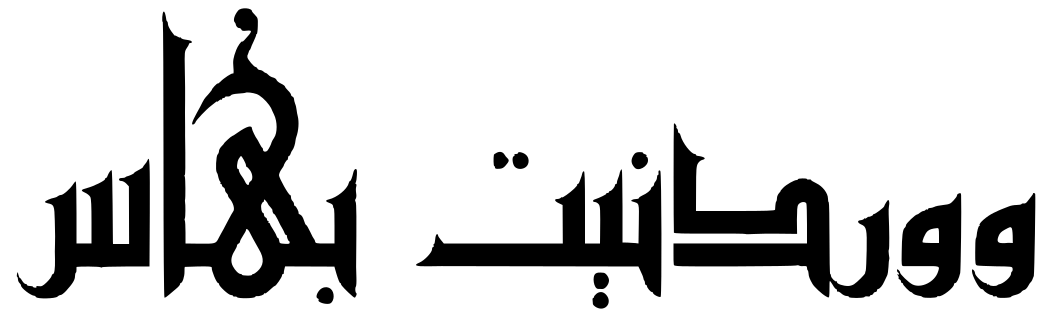
\includegraphics[width=0.5\textwidth]{pics/wnbahasa}
  \\ Wordnet Bahasa
\end{center}
\end{frame}


\begin{frame}{Alphabetic Systems: Malay/Indonesian  --- Rumi}
        \begin{itemize}
        \item Introduced by colonial powers.
          \begin{itemize}
          \item Malay spelling followed English
          \item Indonesian spelling followed Dutch
          \end{itemize}
            \item Standardized in 1972 for both Malaysia and Indonesia.
     \begin{itemize}
  \item \zsm{di-buat} $\rightarrow$ 	\zsm{dibuat}, \zsm{di-rumah} $\rightarrow$ \zsm{di
    rumah}
 \item \zsm{ch} and \zsm{tj} \IPA{/tʃ/}$\rightarrow$ \zsm{c}: \zsm{ketjap/kechap}  $\rightarrow$
    \zsm{kecap}
  \item   \zsm{njonja/nyonya}	 $\rightarrow$ \zsm{nyonya}
  \item   \zsm{ke-barat$^2$-an}	 $\rightarrow$ \zsm{kebarat-baratan}	``westernized''
  \end{itemize}
    \end{itemize}

\end{frame}


\begin{frame}{Alphabetic Systems: Thai}
\begin{itemize}
\item Derived from Old Khmer script.
  \\ Derived from Mon, originally Indic
    \item No spaces between words; consonants represented by main letters, vowels by diacritics.
    \item Example:
    \begin{exe}
    \ex \textthai{สวัสดี} (sawasdee) - Hello
    \end{exe}
    \item Complex relationship between letters and tones.
\end{itemize}
\end{frame}

\begin{frame}{Thai Tones and Consonant Classes}
\begin{itemize}
    \item Consonant letters divided into three classes: high, middle, and low.
    \item Tone determined by initial consonant, tone marks, and vowel length.
    \item Thai words with initial /kh/ (Smalley 1994: 184)\\
      \begin{tabular}{llllll}
        \multicolumn{2}{l}{\textbf{Thai Word}} & \textbf{Meaning} &   \multicolumn{2}{l}{\textbf{Thai Word}} & \textbf{Meaning} \\
        \hline
        \textthai{ขา}& khǎa & leg &       \textthai{คา}& khaa & embedded \\  
        \textthai{ข่า}& khàa & galangal &  \textthai{ค่า}& khâa & cost \\      
        \textthai{ข้า}& khâa & slave &     \textthai{ค้า}& kháa & trade \\     
        \textthai{ขาด}& khàat & lack &    \textthai{คาด}& khâat & to strap \\
        \textthai{ขัด}& khàt & obstruct &  \textthai{คัด} & khát & be clogged \\
     \end{tabular}
     
   \item  Complicated function of the initial consonant, diacritic and final consonant
   \item But generally deterministic
   \item Like most writing systems, sound changes quicker than writing
  \end{itemize}
\end{frame}


\begin{frame}{Thai vowels}
  \includegraphics[width=\textwidth]{pics/thai_vwl_1}
\end{frame}
\begin{frame}{Thai dipthongs}
  \begin{center}
  \includegraphics[height=0.8\textheight]{pics/thai_vwl_2}
\end{center}
\end{frame}

%%% Use Korean
%\koreanfontsf\selectfont

\section{Phonographic Systems: Featural}

\begin{frame}{Korean Hangul}
  \begin{center}
    \includegraphics[height=0.7\textheight]{pics/Hangeul-basic}
  \end{center}
  Image from Wikipedia (2024)
\end{frame}



\begin{frame}{Featural Systems: Korean Hangul}
\begin{itemize}
\item Invented by King Sejong (15th century)
  \begin{itemize}
  \item the process of invention is well documented in the  Hunmin jeongeum, or "The correct sounds for the instruction of the people"
  \end{itemize}
    \item Represents phonemes, arranged in syllable blocks.
    \item Example:
    \begin{exe}
    \ex \textkorean{안녕하세요} \ko[hello]{annyeonghaseyo}
    \end{exe}
  \item It was originally looked down on by scholars (who use hanzi)
    as used by women, children and the uneducated
  \item It was not widely adopted until the 19th century
\end{itemize}
\end{frame}


\begin{frame}{Korean Hangul: Design Principles}
\begin{itemize}
\item Vowels represented by distinct vertical/horizontal strokes.
\item Consonant shapes reflect place of articulation.
\item One syllable is one block
\end{itemize}
\begin{center}
    \includegraphics[height=0.5\textheight]{pics/Jamo_placement}
  \end{center}
Image from Wikipedia (2024), cropped.
\end{frame}

\begin{frame}{Korean Consonants:  shape $\approx$ articulation}

  \begin{center}
  \begin{tabular}{ccc}
\includegraphics[width=0.3\textwidth]{pics/Pronounciation_ㄱ.png} &
\includegraphics[width=0.3\textwidth]{pics/Pronounciation_ㄴ.png} &
\includegraphics[width=0.3\textwidth]{pics/Pronounciation_ㅅ.png} \\
\textkorean{ㄱ} /k/ & \textkorean{ㄴ} /n/ &  \textkorean{ㅅ} /s/ \\
%   \end{tabular}
% \end{center}
% Images from Wikipedia (2024)
% \end{frame}

% \begin{frame}{Korean Consonants:  shape $\approx$ articulation}
%   \begin{center}
%     \begin{tabular}{cc}
 \includegraphics[width=0.3\textwidth]{pics/Pronounciation_ㅇ.png} &
   \includegraphics[width=0.3\textwidth]{pics/Pronounciation_ㅁ.jpg} \\
\textkorean{ㅇ} /ng/ & \textkorean{ㅁ} /m/ \\
    \end{tabular}
    
\end{center}
Images from Wikipedia (2024)
\end{frame}


\begin{frame}{Korean Consonants:  shape $\approx$ articulation}

  \begin{center}
    \begin{tabular}{lcccc}
        & \textbf{Basic} & \textbf{Simple} & \textbf{Aspirated} & \textbf{Tense} \\
        \hline
        Velar & & \textkorean{ㄱ} (\IPA{k}) & \textkorean{ㅋ} (\IPA{kʰ}) & \textkorean{ㄲ} (\IPA{ḳ}) \\
        Fricatives & & \textkorean{ㅅ} (\IPA{s}) & & \textkorean{ㅆ} (\IPA{s͈}) \\
        Palatal &   & \textkorean{ㅈ} (\IPA{tɕ}) & \textkorean{ㅊ} (\IPA{tɕʰ}) & \textkorean{ㅉ} (\IPA{tɕ͈}) \\
        Coronal & \textkorean{ㄴ}  (\IPA{n})& \textkorean{ㄷ} (\IPA{t}) & \textkorean{ㅌ} (\IPA{tʰ}) & \textkorean{ㄸ} (\IPA{t͈}) \\
      Bilabial & \textkorean{ㅁ}  (\IPA{m})& \textkorean{ㅂ} (\IPA{p}) & \textkorean{ㅍ} (\IPA{pʰ}) & \textkorean{ㅃ} (\IPA{p͈}) \\
      \hline
      Dorsal & \textkorean{ㅇ} (\IPA{'}) & \textkorean{ㅇ} (\IPA{ŋ}) &  \textkorean{ㅎ} (\IPA{h}) \\
    \end{tabular}
  \end{center}

\end{frame}


\begin{frame}{Summary}
  \begin{itemize}
  \item Hangul is a well-motivated alphabetic system, not a direct mapping of phonetic features
  \item Many sounds change in combination, so technically it is morphophonemic
  \item It is said that ``A wise man can acquaint himself with them before the morning is over; even a stupid man can learn them in the space of ten days.''
\\ \textit{Hunmin Jeongeum Haerye}, postface of Jeong Inji, p. 27a, translation from Gari K. Ledyard, The Korean Language Reform of 1446, p. 258
  \end{itemize}
  
\end{frame}


\begin{frame}{Cia-Cia}
  \begin{itemize}
  \item  Cia-Cia (Bahasa Ciacia / \textkorean{바하사 찌아찌아})  is a member of the Celebic branch of the Malayo-Polynesian language family (Austronesian)
  \item Spoken by about 80,000 people on Buton Island, a part of Indonesia to the south east of Sulawesi
  \item It used to be written in a Jawi-like script called Gundhul and is now mainly written in Rumi
    
  \item In 2007  Professor Chun Tai-hyun, a professor of Malay and Indonesian linguistics at Hankuk University of Foreign Studies in Seoul developed a Hangeul orthography
    \begin{itemize}
    \item For fricative /v/ it uses the obsolete jamo  \textkorean{ᄫ} 
    \end{itemize}
  \item It was privately taught since 2009 using a textbook written by Lee Ho-young, a linguistics professor at Seoul National University.
  \item It was abandoned around 2012, and revived around 2022 
  \item A Cia-Cia dictionary in Hangul was published in December 2021.
  \item Hangul remains in use in schools and on local signs
\end{itemize}

\end{frame}


\section{Logographic Systems}

\begin{frame}{Chinese Writing System}
\begin{itemize}
    \item Ancient origins, evolved from pictograms.
    \item Continually in use for over 3,000 years
    \item A powerful force for cultural and political unification
    \item Also adopted by surrounding languages (Japanese, Korean, Vietnamese)
    \item Characters mainly represent morphemes, often compound structures.
    \item Example:
    \begin{exe}
    \ex 
    \textchinese{你好} \zh[hello `you good' ]{nǐ hǎo} 
    \ex 
    \textchinese{山} \zh[mountain]{shān}
    \end{exe}
  \item Reformed to simplified characters in the 1950s
\end{itemize}
\end{frame}

\begin{frame}{Development of Chinese character horse \textchinese{马}}

  \begin{center}
  \includegraphics[height=0.85\textheight]{pics/horse-hanzi.eps}    
  \end{center}


\end{frame}

\begin{frame}{Logograph writing system example: Chinese}


  \includegraphics[width=0.9\textwidth]{pics/hanzi-1.eps}
\bigskip

\includegraphics[width=0.9\textwidth]{pics/hanzi-2.eps}
\bigskip

\includegraphics[width=0.9\textwidth]{pics/hanzi-3.eps}


\end{frame}

\begin{frame}{Semantic-phonetic compounds}
 \begin{center}
 \includegraphics[height=0.6\textheight]{pics/hanzi-4.eps}
\end{center}

97\% of Chinese characters are phonetic compounds (Sproat 2010)!  Other estimates are lower (Wang, pc 2013)
\end{frame}

\begin{frame}{Structure of Chinese Characters}
\begin{itemize}
    \item Phonetic component gives clues to pronunciation.
    \item Semantic radical provides meaning hints.
    \item Characters require memorization due to irregular phonetic-semantic correspondences.
\end{itemize}
\end{frame}

\begin{frame}{Using Chinese Characters for Non-Mandarin Chinese}
\begin{itemize}
    \item Chinese characters were designed for Mandarin, which poses challenges for other Sinitic languages.
    \item Problem: Phonetic clues in Mandarin characters often don’t apply to languages like Cantonese and Taiwanese.
    \item For literacy in Cantonese or Taiwanese, familiarity with Mandarin’s written form is often assumed.
    \item Despite differences, some words in Cantonese and Taiwanese can be represented with Mandarin characters.
    \item Issue: Many words and grammatical elements in other Sinitic languages lack standard Mandarin equivalents.
\end{itemize}
\end{frame}

\begin{frame}{Writing Strategies for Cantonese}
\begin{itemize}
    \item Cantonese writers use various strategies to adapt characters:
    \begin{enumerate}
        \item \textbf{Unique Cantonese Characters}: Characters created for words without Mandarin equivalents.
        \item \textbf{Phonetic Resemblance}: Using Mandarin characters that sound similar to Cantonese words.
        \item \textbf{English Letters}: Borrowing letters to represent Cantonese sounds.
    \end{enumerate}
    \item Example of phonetic adaptation: The Cantonese plural suffix \textbf{-deih} is represented by combining ‘mouth’ and ‘earth’ characters, resembling the pronunciation \textbf{deih}: \textyue{哋}
\end{itemize}
\end{frame}


\begin{frame}{Workarounds}


  \begin{exe}
  \ex
  \glll 你	喺	{嗰	喥}	好	喇,	千	祈	咪	搞	佢	啲	嘢 。 \\
	你	o係	{果	度}	好	la,	千	祈	咪	搞	佢	D	野 。 \\
        you	being	there	good	SFP,	thousand	pray	don't	{mess with}	he/she	of	things/stuff . \\
        \trans You'd better stay there, and under no circumstances mess with his/her stuff.
      \end{exe}
      \begin{itemize}
      \item use 'o' instead of \textyue{口}
      \item use alphabet: 'D'
      \item use homophones: 	\textchinese{果	度} for \textyue{嗰 喥}
      \item because Cantonese is mainly spoken, there is considerable
        variation in the orthography
      \end{itemize}
    \end{frame}

\begin{frame}{Loan words}

Because of the influence of English, Cantonese tends to use more loan words (as does Singapore Mandarin).  Note that speakers also freely use Mandarin vocabulary, \ldots

\begin{center}
\begin{tabular}{llllll}

  Cantonese & Jyupting &  English & Mandarin & Pinyin\\
  \hline
\textyue{BB} & bi4 bi1 &baby & \textchinese{嬰兒} & ying1 er2\\
\textyue{巴士} & baa1 si2 & bus & \textchinese{公交车} & gong1 jiao1 che1\\ 
\textyue{拜拜} & baai1 baai3  & bye bye & \textchinese{再见} & zai4 jian4 \\
\textyue{沙展} & saa1 zin2 & sergeant & \textchinese{排长} & pai2 zhang3 \\
\end{tabular}
\end{center}
\end{frame}


    
\section{Japanese: A Multiscript System}
\begin{frame}{Japanese Writing System}
\begin{itemize}
    \item Combines kanji (logographic) and kana (syllabic).
    \item Example:
    \begin{exe}
    \ex \begin{tabbing}
    \textjapanese{こんにちは} \= konnichiwa \= (hello) \\
    \textjapanese{山} \> yama \> (mountain)
    \end{tabbing}
    \end{exe}
\end{itemize}
\end{frame}

\begin{frame}{Syllabaries: Hiragana and Katakana}
\begin{itemize}
    \item Hiragana: Used for particles, auxiliary verbs, and suffixes.
    \item Katakana: Used for loanwords, mimetics, and emphasis.
    \item Example syllabary table for Hiragana and Katakana.
\end{itemize}
\end{frame}




\begin{frame}{Hiragana - a true syllabic alphabet} 
% Script developed in 10th century from Chinese characters. 52 characters.

% %Hiragana were originally called onnade or 'women's hand' as were used
% %mainly by women - men wrote in kanji and katakana. By the 10th
% %century, hiragana were used by everybody.
\begin{center}
   \includegraphics[height=0.8\textheight]{pics/hiragana.png}
\end{center}

\end{frame}
\begin{frame}{Katkana - a true syllabic alphabet} 
% Script developed in 10th century from Chinese characters. 52 characters.

% %Hiragana were originally called onnade or 'women's hand' as were used
% %mainly by women - men wrote in kanji and katakana. By the 10th
% %century, hiragana were used by everybody.
\begin{center}
   \includegraphics[height=0.8\textheight]{pics/katakana.png}
\end{center}

\end{frame}

\begin{frame}{Extending Hiragana and Katakana}

  \begin{itemize}
    \item \txx{Dakuon} (\textjapanese{濁音: ゛}): voicing
     \begin{itemize}
     \item        \textjapanese{か} (ka) → \textjapanese{が} (ga);
     \item       \textjapanese{さ} (sa) → \textjapanese{ざ} (za);
     \item       \textjapanese{た} (ta) → \textjapanese{だ} (da);
     \item      \textjapanese{ハ} (ha) → \textjapanese{バ} (ba)
     \end{itemize}
   \item \txx{Handakuten} (\textjapanese{半濁点: ゜}) plosive
      \begin{itemize}
      \item \textjapanese{は} (ha) → \textjapanese{ぱ} (pa)
    \end{itemize}
 \item \txx{Yōon} (\textjapanese{拗音}): palatized
   \begin{itemize}
   \item Consonant + 'i' combines with small "ya," "yu," or "yo"
      (\textjapanese{ゃ}, \textjapanese{ゅ}, \textjapanese{ょ}).
     \begin{itemize}
     \item      \textjapanese{き} (ki) + \textjapanese{ゃ} (xya) → \textjapanese{きゃ} (kya); 
     \item \textjapanese{し} (shi) + \textjapanese{ょ} (xyo) → \textjapanese{しょ} (sho); \ldots
     \end{itemize}
     %   %     % \item In katakana: \textjapanese{キ} (ki) + \textjapanese{ャ} forms 
  % \\    \textjapanese{キャ} (kya); \textjapanese{シ} (shi) + \textjapanese{ョ} forms \textjapanese{ショ} (sho).
   \end{itemize}
 \item \txx{GōYōon} (\textjapanese{合拗音 }): labialized (now only in Okinawan)
    \begin{itemize}
    \item  \textjapanese{くゎ} (kwa),  \textjapanese{くゐ} (kwi),
      \textjapanese{くゑ} (kwe),  \textjapanese{くを} (kwo)
   \end{itemize}
 \item \txx{Sokuon} (\textjapanese{促音}):
   \begin{itemize}
   \item Small \textjapanese{っ} marks a geminate consonant
     \\ normally transliterated by doubling \textjapanese{さっか} \jpn{sakka}
   \end{itemize}
 \end{itemize}
\end{frame}


\begin{frame}{Kanji and Mixed System Writing}
\begin{itemize}
    \item Lexical roots written in kanji.
    \item Grammatical elements in hiragana.
    \item Foreign words in katakana (or romaji).
    \item Mixed system allows nuanced text creation.
    \end{itemize}
    \begin{exe}
      \ex \glll 彼女 は T シャーツ を 着.て いる \\
      kanojo ha T sha-tu wo {ki te} iru \\
      she TOP T shirt ACC wear PRG  \\
      \trans She is wearing a T-shirt
    \end{exe}

    
\end{frame}


\begin{frame}{Homophones and Context Dependence}
\begin{itemize}
    \item Japanese has many homophones due to the limited set of sounds in the language.
    \item Kanji helps distinguish words with the same pronunciation but different meanings, yet:
    \begin{itemize}
        \item Words with identical readings may use different kanji.
        \item Context often determines which kanji is appropriate, adding complexity.
    \end{itemize}
    \item Example: \textjapanese{こうしょう} (kōshō) can mean "negotiation" (\textjapanese{交渉}) or "factory" (\textjapanese{鉱床}), depending on kanji and context. (WWWJDIC has 44 possible entries)

\end{itemize}
\end{frame}

\begin{frame}{Why Kanji Have Multiple Readings}
\begin{itemize}
    \item Kanji have multiple readings due to their integration from Chinese into Japanese over centuries.
    \item Japanese and Chinese are linguistically different, so adaptations were necessary.
    \item Kanji readings can be divided into two main types:
    \begin{itemize}
        \item \textbf{On’yomi} (\textjapanese{音読み}): Chinese-derived readings.
        \item \textbf{Kun’yomi} (\textjapanese{訓読み}): Native Japanese readings.
    \end{itemize}
    \item This dual system has led to multiple ways of reading kanji, depending on context.
\end{itemize}
\end{frame}

\begin{frame}{Historical Borrowing from Chinese}
\begin{itemize}
    \item Kanji were imported from China starting in the 5th century, with Chinese pronunciations.
    \item \textbf{On’yomi} (\textjapanese{音読み}) readings were derived from Chinese pronunciations.
    \item Different periods and regions of Chinese influence led to varied on’yomi.
    \item For example, \textjapanese{山} has the reading \textjapanese{さん} ("san") in compounds, like in \textjapanese{火山} ("kazan," meaning "volcano").
    \item The Chinese-derived readings are often used in compound words.
\end{itemize}
\end{frame}

\begin{frame}{Native Japanese Words (Kun’yomi)}
\begin{itemize}
    \item Many kanji represented concepts that already had native Japanese words.
    \item To adapt, kanji were assigned \textbf{kun’yomi} (\textjapanese{訓読み}), or native Japanese readings.
    \item Example: \textjapanese{明} can be read as \textjapanese{あか} in  the native Japanese word  明るい \jpn[bright]{akarui}.
    \item Kun’yomi is often used when kanji stand alone or in names.
    \item This creates another layer of readings that are essential for native vocabulary.
    \item Many characters also have readings normally only used in names \textbf{nanori} (\textjapanese{名乗り})
\end{itemize}
\end{frame}

\begin{frame}{Multiple Chinese Influences: Go-on, Kan-on, Tō-on}
\begin{itemize}

    \item Kanji were imported from China starting in the 5th century, with Chinese pronunciations.
    \item \textbf{On’yomi} (\textjapanese{音読み}) readings were derived from Chinese pronunciations.
    \item Kanji were borrowed in waves, reflecting different Chinese dynasties and regions:
    \begin{itemize}
        \item \textbf{Go-on} (\textjapanese{呉音}): Earlier readings from the Wu region.
        \item \textbf{Kan-on} (\textjapanese{漢音}): Pronunciations from the Tang Dynasty.
        \item \textbf{Tō-on} (\textjapanese{唐音}): Later readings from the Song and Ming Dynasties.
    \end{itemize}
    \item Some kanji have multiple on’yomi due to these varied influences, used in different contexts.
    \item Example: \textjapanese{明} has readings like \textjapanese{めい} ("mei") and \textjapanese{みょう} ("myō") based on context.
\end{itemize}
\end{frame}

\begin{frame}{\textjapanese{明}}

  According to Kanjidic this character has the following readings:
  \begin{itemize}
  \item ON:  \textjapanese{メイ ミョウ ミン}
  \item KUN: \textjapanese{あ.かり あか.るい あか.るむ あか.らむ あき.らか あ.ける -あ.け あ.く あ.くる あ.かす}
  \item Names: \textjapanese{あきら あけ あす きら け さや さやか とし はる み め} 
  \end{itemize}
  
  \url{https://www.edrdg.org/cgi-bin/wwwjdic/wwwjdic?1B}

  Chinese and Korean have one reading each \zh{ming2} and \ko{myeong}
  
\end{frame}


% \begin{frame}{Compound Words and Contextual Adaptations}
% \begin{itemize}
%     \item Kanji are often combined to form compound words (\textjapanese{熟語}), where readings can vary.
%     \item Example: \textjapanese{生} can be read as \textjapanese{せい} ("sei"), \textjapanese{しょう} ("shō"), or \textjapanese{なま} ("nama") depending on context.
%     \item Some compounds mix \textjapanese{音読み} (on’yomi) and \textjapanese{訓読み} (kun’yomi) within the same word.
%     \item Over time, certain kanji took on additional meanings, adding even more readings.
%     \item Context, pronunciation, and historical use all influence which reading is appropriate.
% \end{itemize}
% \end{frame}


\begin{frame}{Character Complexity and Memory Load}
\begin{itemize}
    \item Japanese kanji characters are often complex and require memorization of many details:
    \begin{itemize}
        \item A standard-educated adult in Japan knows about 2,000 kanji.
        \item Each kanji has multiple readings (pronunciations), which change based on context and word combinations.
    \end{itemize}
    \item Learning kanji is time-intensive, requiring years of study.
    \item Even native speakers may struggle with less common kanji or readings, leading to a heavy memory load.
\end{itemize}
\end{frame}

\begin{frame}{Historical Reforms and Modern Challenges}
\begin{itemize}
    \item Orthographic reforms have been implemented to simplify kanji, but challenges remain:
    \begin{itemize}
        \item The \textbf{Tōyō Kanji} reform (1946) and \textbf{Jōyō Kanji} list (1981) aimed to standardize kanji usage.
        \item However, non-standard or rare kanji still appear in literature and names, requiring additional study.
    \end{itemize}
    \item Modern technology poses new issues:
    \begin{itemize}
        \item Typing kanji requires selecting the correct character from multiple homophones.
        \item Many younger people may rely on digital aids, impacting kanji writing skills.
    \end{itemize}
    \item These factors continue to make Japanese orthography a challenging system to master.
\end{itemize}
\end{frame}

\section{Calligraphy}
\begin{frame}{Calligraphy in East Asia}
\begin{itemize}
    \item Highly valued art form, more esteemed than painting.
    \item Reflects cultural aesthetics and individuality.
    \item Styles include Seal Script, Clerical Script, Standard Script, Running Script, and Grass Script.
    \item Chinese calligraphy emphasizes brush techniques and stroke order.
\end{itemize}
\begin{center}
    \begin{tabular}{cc}
      \includegraphics[height=0.5\textheight]{pics/This_Letter_written_by_Mi_Fei.jpg} &
                                                                                        \includegraphics[height=0.5\textheight]{pics/Songhuizong.jpg} \\
      
      Mi Fu (1051–1107) & Emperor Huizong of Song (1082–1135)
    \end{tabular}
  \end{center}
\end{frame}

\begin{frame}{Japanese Calligraphy}
\begin{itemize}
    \item Emphasis on the beauty of handwriting.
    \item Grass style and Zen calligraphy notable for their fluidity and abstraction.
\end{itemize}
\begin{center}
  \begin{tabular}{cc}
 \includegraphics[height=0.5\textheight]{pics/Muso_Soseki_3.jpg} & \includegraphics[height=0.5\textheight]{pics/Shodo+Ichigo+Ichinen.jpg}\\
  \textjapanese{別無工夫} &  \textjapanese{一期一会} \\
 \jpn{betsu-naku kuufuu} & \jpn{ichi-go ichi-e}   \\ 
  nothing else but focus &  one lifetime one chance                                             
  \end{tabular}
    \end{center}
\end{frame}


\begin{frame}{Indonesian Calligraphy}
\begin{itemize}
    \item Jawi calligraphy is based on Arabic calligraphy
    \item Often very ornate
      
\end{itemize}
\begin{center}
\includegraphics[height=0.5\textheight]{pics/jawi-calligraphy.jpeg}
\end{center}
\end{frame}

\begin{frame}{Arabic calligraphy in Diwani style}

\begin{center}
\includegraphics[height=0.5\textheight]{pics/Diwani_Izzet_al_Karkuki.jpg} \\
\textarabic{يَا أَيُّهَا النَّبِيُّ إِنَّا أَرْسَلْنَاكَ شَاهِدًا وَمُبَشِّرًا وَنَذِيرًا وَدَاعِيًا إِلَى اللَّهِ} \\
"O Prophet, indeed We have sent you as a witness and a bringer of good tidings and a warner, and as one who invites to Allah." \\ 


Mehmet Izzet al-Karkuki (1841-1904)
\end{center}

\href{https://en.wikipedia.org/wiki/Diwani}{Diwani} is a calligraphic variety of Arabic script, developed during the reign of the early Ottoman Turks (16th century - early 17th century).
\end{frame}


\begin{frame}{Acknowledgements}

  \begin{itemize}
  \item Images taken from  Omniglot (\url{https://omniglot.com/}) unless otherwise stated
  \end{itemize}
  
\end{frame}


\end{document}

%%% Local Variables: 
%%% coding: utf-8
%%% mode: latex
%%% TeX-PDF-mode: t
%%% TeX-engine: xetex
%%% End: 
